%
% ddg.tex
%

A data-driven game \cite{10} separates game content from the game code. This design allows both game programmers and game designers (groups with very different skillsets) to contribute separately to game development. This separation has long been practiced, for example by storing models, textures and sounds in data files separate from the game engine; this trend has recently accelerated by trying to move as much content as possible out of the engine: character and story-line data is increasingly \cite{25} being stored in external configuration files. Modern design goes even further, storing game logic specific to game play in external files written in a scripting language such as Lua, Python or a custom-made scripting language \cite{SCRIPTING_LUA,SCRIPTING_PYTHON,UNREALSCRIPT_LATENT_FUNCTIONS}.

\begin{figure*}
\begin{center}
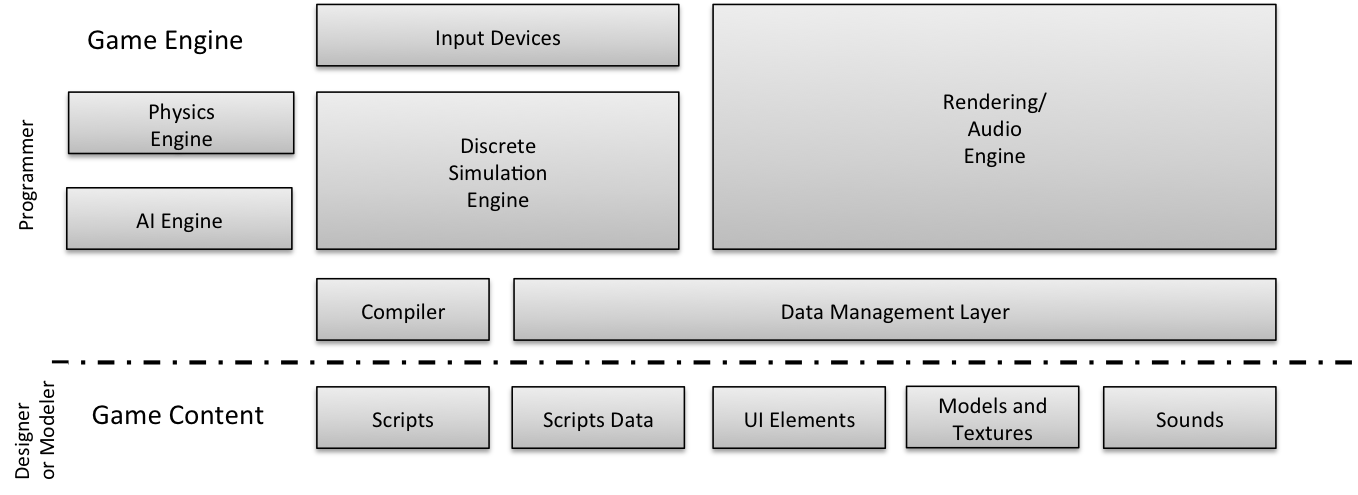
\includegraphics[scale=0.5]{engine_architecture.png}
\end{center}
\label{fig:data_driven_games}
\caption{Data-driven game architecture}
\end{figure*}

In Figure 2 we can see the general architecture of a data-driven game. The game engine (AI, physics, rendering, audio and discrete simulation) is written and maintained by programmers. Typically, the discrete simulation engine puts together the interactions between physics, AI and game logic in a meaningful way, and exposes the resulting game state and events to the rendering and audio engine which give some feedback to the player. The game content is created by game designers, who are responsible with creating and populating the game world; the game world contains both artistic elements like models and sounds, but also logical elements such as behaviors and character statistics. Logical elements are defined by scripts; scripts are either compiled or interpreted and executed by the discrete simulation engine. Separating scripts becomes important in all those game where character behavior must be tested and adjusted constantly during development to ensure that there is no single optimal strategy that can ensure victory (otherwise the game would lose much of its challenge and interest). Also, separating game logic into scripts allows for ``modding'', that is players can modify the game even without access to its source code; the creativity of the players can extend the lifetime of a game beyond the original intentions of its developers (\cite{21}). The entire focus of the authors is on the discrete simulation engine and how techniques taken from the database comunity can be used to build a better performing implementation that can be heavily scripted.

\paragraph{The Discrete Simulation Engine}
Game are processed in clock ticks. During each clock tick the simulation engine processes the current state of the world, thereby computing its updated version. This usually consists in considering the actions of all the characters of the game (some characters may perform null actions, but still they are given an opportunity at every tick); each action may produce several \textit{effects}.  Effects produced during the same tick are written into the game state simultaneously, allowing us to cleanly separate each clock tick into three stages:

\begin{itemize}
\item a query stage when we read the contents of the game data
\item a decision stage where we choose the actions of each character
\item an update stage where we write into the game state the effects produced by each action
\end{itemize}

Since actions are all updating the game data simultaneously, we use a transaction model to describe how these updates are processed. Since effects usually increase or decrease numeric values then such a model becomes simply an aggregate function such as \texttt{(+), (-), max, min, ...}. Effects are usually separated into \textit{stackable} and \textit{non-stackable}, depending on whether or not they accumulate during one tick or only one update is picked; for example, damage is stackable since a unit that suffers damage from multiple opponents receives the sum of all these damages, while healing auras are non-stackable because only the most beneficial aura is applied while all the others are discarded.